\section{Micro-Cell Models and Optimization Scenarios}
\label{sec:63models}

\minitoc{62mm}{3}

\noindent
In the following, we present the different micro-cell models
and optimization scenarios for which we perform numerical
experiments in the next section.



\subsection{Micro-Cell Models}
\label{sec:631models}

We use the various micro-cell models that are depicted in \cref{fig:microCell}.
The models differ in the spatial dimensionality $\dimobjdomain$
and the number $d$ of micro-cell parameters
$\*x \in \clint{\*0, \*1} = \clint{0, 1}^d$.
Note that the presented models are only some examples.
One can easily design complicated micro-cell models
with larger numbers of parameters.

\begin{figure}
  \subcaptionbox{%
    \lefthphantom{2D cross}{(2D-C, $d = 2$)}\\(2D-C, $d = 2$)%
    \label{fig:microCell_1}%
  }[31mm]{%
    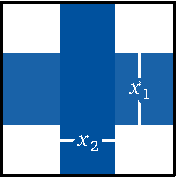
\includegraphics{microCell_1}%
  }%
  \hfill%
  \subcaptionbox{%
    2D framed cross\\(2D-FC, $d = 4$)%
    \label{fig:microCell_2}%
  }[31mm]{%
    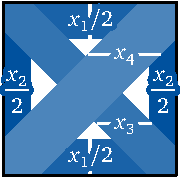
\includegraphics{microCell_3}%
  }%
  \hfill%
  \subcaptionbox{%
    2D sheared cross\\\rlap{\hspace*{11mm}{(2D-SC, $d = 3$)}}%
    \label{fig:microCell_3}%
  }[41mm]{%
    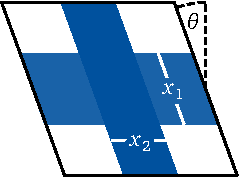
\includegraphics{microCell_2}%
  }%
  \hfill%
  \subcaptionbox{%
    2D sheared framed cross (2D-SFC, $d = 5$)%
    \label{fig:microCell_4}%
  }[37.5mm]{%
    \hspace*{-45mm}%
    \rlap{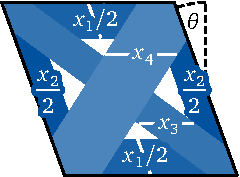
\includegraphics{microCell_4}}%
  }\\[2mm]%
  \subcaptionbox{%
    3D cross (3D-C, $d = 3$)%
    \label{fig:microCell_5}%
  }[44mm]{%
    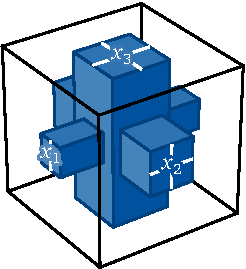
\includegraphics{microCell_5}%
  }%
  \quad%
  \subcaptionbox{%
    3D sheared cross (3D-SC, $d = 5$)%
    \label{fig:microCell_6}%
  }[56mm]{%
    \hspace*{5mm}%
    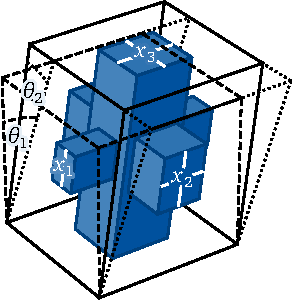
\includegraphics{microCell_6}%
  }%
  \caption[Types of micro-cell models]{%
    Types of micro-cell models in two dimensions \emph{(top row)}
    and three dimensions \emph{(bottom row)}.%
  }%
  \label{fig:microCell}%
\end{figure}

\paragraph{Orthogonal (non-sheared) models in two dimensions}

The basic component of the four two-dimensional models
is a square with a cross (\cref{fig:microCell_1})
of two axis-aligned orthogonal bars,
whose widths are determined by two micro-cell parameters $x_1$ and $x_2$.
The micro-cell parameters are ratios of the bar widths
to the edge lengths of the micro-cell
(although the actual micro-cells are infinitesimally small).
This results in the \emph{cross model.}
For the \term{framed cross model} (\cref{fig:microCell_2}),
we add a diagonal cross with orthogonal bars
of widths $x_3$ and $x_4$ (horizontally measured).
To simplify the boundary treatment,
we shift the contents of the framed cross micro-cell by
\SI{50}{\percent} of the micro-cell's edge lengths in both directions,
such that previous corners of the micro-cell correspond to the new center.

\paragraph{Sheared models in two dimensions}

Both of these models can be extended by shearing.
The idea is to increase the stability of the resulting macro-structure
with respect to forces that act at angles other than
\ang{0} and \ang{90} (cross model) or
\ang{0}, \ang{90}, and \ang{45} (framed cross model).
If we just rotated the crosses in the micro-cells,
then the micro-structure would not be periodic.
Instead, we shear the whole micro-cell in the horizontal direction,
where the shearing angle $\theta$ is an additional micro-cell parameter,
which gives us another degree of freedom.%
\footnote{%
  To be more precise, the angle $\theta$ corresponds to an
  additional micro-cell parameter $x_3$ (sheared cross) or
  $x_5$ (sheared framed cross) that is determined by normalization
  from $\clint{-0.35\pi, 0.35\pi}$, i.e., $\theta/(0.7\pi) + 1/2$.%
}
This results in the \term{sheared cross model} (\cref{fig:microCell_3})
and \term{sheared framed cross model} (\cref{fig:microCell_4})
with three and five micro-parameters each.

\paragraph{Models in three dimensions}

The two-dimensional cross model can be transferred to three
spatial dimensions by just adding another bar in the new dimension.
Each of the three bars has square cross-section with given edge lengths
$x_1$, $x_2$, or $x_3$, respectively,
resulting in the \term{3D cross model} with three micro-cell parameters
(\cref{fig:microCell_5}).
By shearing in the two horizontal directions,
we obtain two new degrees of freedom $\theta_1$ and $\theta_2$
(shearing angles).
The emerging \term{3D sheared cross model} has five micro-cell parameters
(\cref{fig:microCell_6}).



\subsection{Test Scenarios}
\label{sec:632scenarios}

To benchmark the performance of the new method,
we take a subset of the scenarios given in \cite{Valdez17Topology},
which reviews more than 100 papers on topology optimization
to determine the most common test scenarios in the field.
The geometry and the boundary conditions of the
four scenarios (two for each 2D and 3D)
are given in \cref{fig:topoOptScenario} (dimensions in meters).
In contrast to \cite{Valdez17Topology},
we only use single-point loads
(i.e., not loads applied to line segments, areas, or volumes)
for implementational reasons.
The upper bound on the density (see \cref{sec:611homogenization})
is $\densub = \SI{50}{\percent}$ for the 2D scenarios and
$\densub = \SI{10}{\percent}$ for the 3D scenarios.
As in \cite{Sigmund01Line} and for reasons of simplicity,
we apply a force $\force$ with unit value
(i.e., $\norm[2]{\force} = \SI{1}{\newton}$),
and we use a hypothetical material with
a Young's modulus (stiffness) of \SI{1}{\pascal} and
a Poisson ratio (transversal expansion to axial compression) of $0.3$.

\begin{figure}
  \subcaptionbox{%
    2D cantilever%
    \label{fig:topoOptScenario_1}%
  }[72mm]{%
    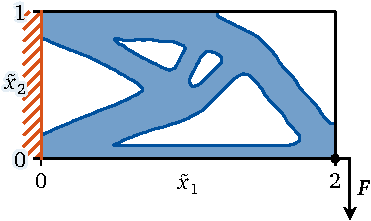
\includegraphics{topoOptScenario2D_1}%
  }%
  \hfill%
  \smash{\raisebox{-22mm}{\subcaptionbox{%
    2D L-shape%
    \label{fig:topoOptScenario_2}%
  }[72mm]{%
    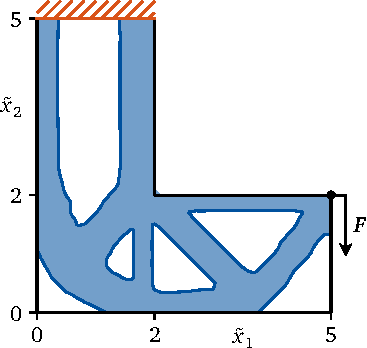
\includegraphics{topoOptScenario2D_2}%
  }}}%
  \\[7mm]%
  \subcaptionbox{%
    3D cantilever%
    \label{fig:topoOptScenario_3}%
  }[72mm]{%
    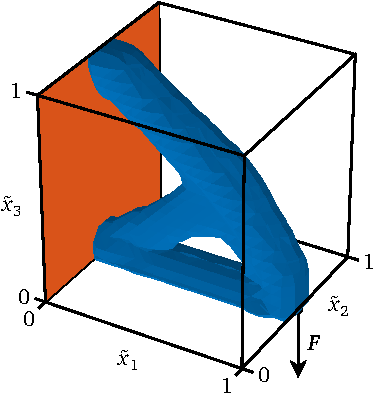
\includegraphics{topoOptScenario3D_1}%
  }%
  \hfill%
  \subcaptionbox{%
    3D center-load%
    \label{fig:topoOptScenario_4}%
  }[72mm]{%
    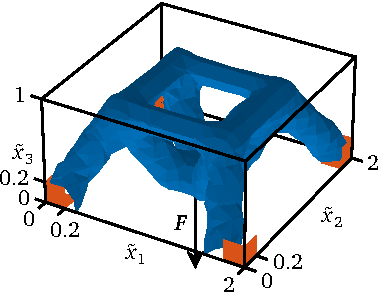
\includegraphics{topoOptScenario3D_2}%
  }%
  \caption[Test scenarios in topology optimization]{%
    Test scenarios in topology optimization in
    two and three spatial dimensions.
    Shown are
    the domains $\objdomain$,
    load points,
    locations of homogeneous Dirichlet boundary conditions
    \emph{\textcolor{C1}{(red)},} and
    exemplary optimal structures \emph{\textcolor{C0}{(blue)}.}%
  }%
  \label{fig:topoOptScenario}%
\end{figure}
